\subsection{Multiple Translation Units [Simone]}
\label{sec:Insieme.Frontend.TranslationUnits}

INSPIRE represents input programs as a whole. This opposes to the way C programs
are usually written, by splitting the entire program into multiple files or
\emph{translation units}. In the trivial case when the entire program is
contained into a single source file, then the generation of the INSPIRE program
can be generated by examining that single file.

\begin{figure}[tb]
	\centering
	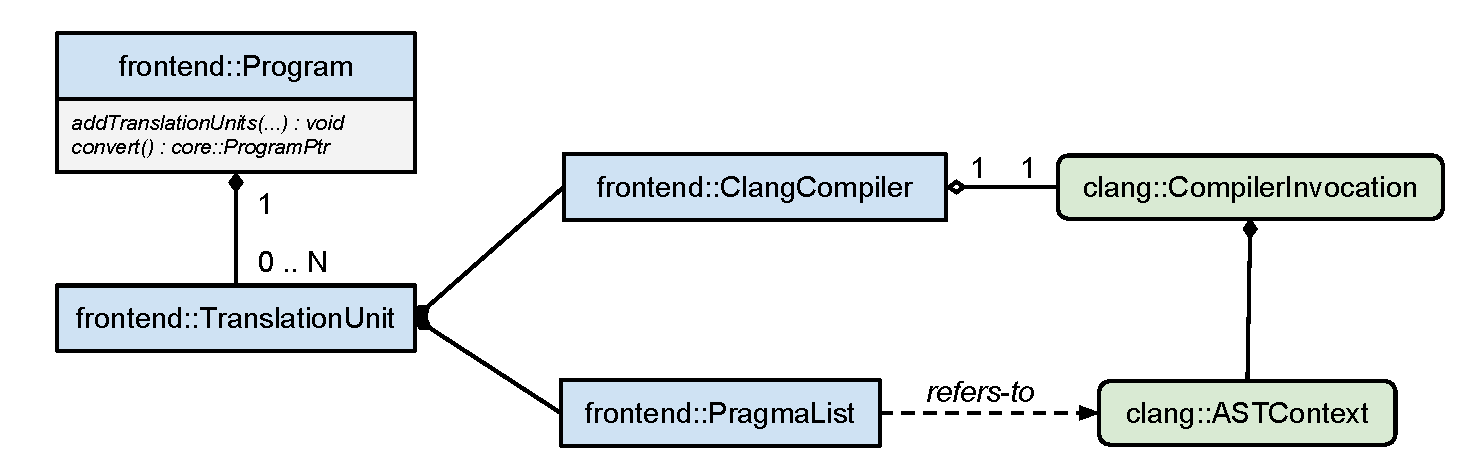
\includegraphics[width=\textwidth]{compiler/frontend/tran_units.pdf}
	\caption{Class Diagram of the Frontend's entry point}
	\label{fig:Frontend.Translation.Units}
\end{figure}

\subsubsection{{\tt LLVM/Clang} Compiler Wrapper}

The Insieme frontend is shaped around the {\tt LLVM/Clang} compiler which
provides the utilities to perform syntactic and semantic analysis on the input
code. Because of performance reasons, the {\tt LLVM/Clang} compiler parses
translation units separately.  An instance of the {\tt LLVM/Clang} compiler
takes care of converting a C/C++ input file into an AST which is internally
represented by an object of the class \type{clang::ASTContext} 
{\tt [\url{http://clang.llvm.org/doxygen/classclang_1_1ASTContext.html}] }. 
In order to simplify the instantiation of {\tt LLVM/Clang} compiler instances,
the Insieme frontend implements a wrapper, \type{ClangCompiler} defined in the
\file{frontend/compiler.h} header providing a simple way of retrieving a {\tt
LLVM/Clang} AST from an input file. The class uses the PIMPL design pattern to
hide implementation details as much as possible to the consumer of this class.
The code which deals with the instantiation of a Clang compiler instance and the
setup of compilation flags being forwarded to Clang is isolated in the
\file{frontend/compiler.cpp} file. In the implementation code of the
\type{ClangCompiler} class we make sure that system include paths are correctly
set both for C and C++ headers. Several other flags are forwarded from the
Insieme input flags. 

\subsubsection{Storing Translation Units}

The \type{ClangCompiler} contains the AST generated by the {\tt LLVM/CLang}
compiler. When the instance of this class is destroyed also the associated
\type{clang::ASTContext} is lost. Therefore it is important to keep alive
instances of the \type{ClangCompier} class until the conversion of the input
program to IR code is completed. Together with the AST of a translation Insieme
can also store additional data structures which refer to the translation unit
for later use. An example is the content of user pragmas within the input code.
Because {\tt LLVM/Clang} is not capable of store the information on user
pragmas, during the generation of AST we store all the pragmas into a separate
data structure \type{frontend::pragma::PragmaList} which contains the list of
pragmas in the current translation unit; where each pragma points to the AST
statement it was associated to. Once a translation unit is processed, all the
information are stored in the \type{frontend::TranslationUnit} class. 

\subsubsection{Frontend's Main Entry Point}

The task of keeping alive translation units is performed by the
\type{frontend::Program} class defined in \file{frontend/program.h}. Also this
class uses the PIMPL design pattern to hide its implementation details. The
interface of this is the main entry point of the Insieme frontend. The
constructor of the \type{Program} class accept a \type{core::NodeManager}, which
will be used during the conversion from C to IR.  The method
\decl{addTranslationUnit(const std::string\& file)} has the purpose of loading
the AST of the {\tt file} into memory. When all translation units are loaded,
the \type{convert()} function triggers the conversion of the input program into
an IR DAG. 

An example of how to manually instantiate the frontend: 
\begin{srcCode}
using namespace insieme;

using core::NodeManager;
using frontend::Program;

NodeManager mgr;
Program p(mgr);
p.addTranslationUnits( {"file1.c", "file2.c"} );
// Use the settings provided by he input line arguments 
core::ProgramPtr ir = p.convert();
\end{srcCode}

This way of initializing the frontend requires command line options, which for
example contains the list of include folders and preprocessor definitions, to be
previously set (see \ref{Command.Line.Args}). Another way of invoking the
frontend overwriting the values set via command line options is
provided by the \type{frontend::ConversionJob} \emph{facade} defined in
\file{frontend/frontend.h}.

\begin{srcCode}
using namespace insieme;

using core::NodeManager;
using frontend::ConversionJob;

NodeManager mgr;
ConversionJob job(mgr, {"file1.c", "file2.c"}, {".", "/usr/include"});
// Enable OpenMP support
job.setOption(frontend::ConversionJob::OpenMP, true);
core::ProgramPtr ir = job.execute();
\end{srcCode}

When a new translation unit is add, the parser of the {\tt LLVM/Clang} compiler
is invoked on that file and AST is generated. This action is triggered by the
constructor of a \type{TranslationUnitImpl} object which is defined in
\file{frontend/program.cpp}. The constructor of this class takes care of
registering pragma handler (see Section~\ref{sec:Insieme:Pragmas}) and starting
the parser which perform syntactic and semantic checks on the input code. If the
translation unit contains no errors, the \type{clang::ASTContext} object is
returned. 

The next operation performed on the AST associated to the translation unit is
\emph{indexing}. Indeed, because during the IR generation we need to be able to
retrieve, by name, symbols which may have been defined in a different
translation units we need to generate an index, or symbol table, which allows us
to easily find definitions given a name. Fortunately, the {\tt LLVM/Clang}
compiler provide an indexing utility \type{clang::idx::Index}.

\subsubsection{Symbol Index and Function Call Graph}
Once every translation unit is loaded, and the index is populated the last
action before the conversion starts is to locate the main entry point of the
input program. Insieme (at this development stage) can only correctly deal with
input codes having an entry point. For example, Insieme cannot be used to
compiler a library code. The reason is mostly connected with the design
of the IR which enforces restrictions on the way global and static variables are
used. We cover this aspect in detail in the next
Section~\ref{sec:Insieme.Frontend.Global}. In order to locate the entry point of
the input code we generate the whole call-graph of and then locate the entry
point. This is done using the \type{clang::CallGraph} utility provided by the
{\tt LLVM/Clang} compiler. If the input program has not entry point, the
frontend launch an exception and quite the compilation process. If the main
entry point is present, then the C/C++ to IR conversion is started. 

\subsubsection{Implications}
The way Insieme handle multiple translation units has several implication on
what Insieme ``can'' and ``cannot'' do. For example, when compiling a big
project via a {\tt Makefile} it {\bf WILL NEVER} be possible to replace the {\tt
CC} and {\tt CXX} environment variables to point to the Insieme executable and
run {\tt make}. As already stated, Insieme needs all the translation units of
the input program to be specified before the conversion to INSPIRE can be
performed. 

Two strategies can be used to compile programs with multiple translation units 
in Insieme. The former is to list all the source files composing the input
program when the Insieme compiler is launched. 

\begin{verbatim}
$> insiemec file1.c file2.c file3.c main.c 
\end{verbatim}

This solution works with small programs, however fails for large codes for
several reasons. First of all, it requires to list all the files of the input
program which depending on the complexity of the project could be located in
several paths. Additionally, real codes usually do not compile all the source
codes in the {\tt src} folder but depending on user-provided compilation flags
choose a version of a file instead of another. Often trying to compile all
source files in a project will result in a compilation error (even when a
standard C/C++ compiler is utilized). 

A more appealing strategy which can be used in such scenarios is to trick the
{\tt make} command and instead of letting him produce a binary file, let it put
together all the source code of the input program into a single file. The
output of the main will be a huge blob of source code which will contain a main
entry point and therefore can be handled by Insieme. This solution is in
practice very easy to be applied. First of all instead of running the host
compiler on every translation unit, let make run only the preprocessor. In this
way all the preprocessor macros are taken care of and the output file will be a
source code where all the headers and macros have been expanded. In order to do
this set the {\tt CC} or {\tt CXX} compiler to {\tt gcc -E}. Notice that the
object files {\tt .o} generated for each translation units will now be source
code. The last step of the makefile is to run the linker. Because the linker
expects object files, and instead we have source files we need to replace the
linker command with an utility which merges together the source code into a
single output file. This might be more complex than expected as the make file
often uses the {\tt CC} variable also as a linker. In this case the linker will
fail because GCC assumes the {\tt .o} files are object files and it will not be
able to perform any operation on those files. If you are able to locate the
linking command in the Makefile, you can replace the {\tt LD} variable with a
merging utility like the following:

\begin{lstlisting}
#! /bin/sh
""":"
exec python $0 ${1+"$@"}
"""
from optparse import OptionParser
import shutil

parser = OptionParser()
parser.add_option("-o", "--output", dest="out", help="output filename", metavar="FILE")
(options, args) = parser.parse_args()

out_file = options.out
for obj_file in args:
	shutil.copyfile( obj_file, out_file )
\end{lstlisting}

The output file of the make will be an executable which contains the entire
application source code. This singol file can be fed to Insieme and let the
magic happen.

